\section*{Problem 3 - State estimation using a Kalman filter}


\subsection*{Problem 3.a} 
\textbf{Describe the purpose of the matrices \textbf{Q}, \textbf{R} and \textbf{P}  in the Kalman filter and state their dimension. }

The matrix  \textbf{Q} is the covariance matrix of the process noise $\omega$ while the matrix \textbf{R} is the covariance matrix of the meausrement noise $v$. 

\begin{align}
    dim(R) = 2\times2 \\
    dim(Q) = 4\times4 
\end{align}

The dimension of \textbf{Q} is $5\times5$ if we include the aileron. \\ 
$P$ is the state estimation error covariance matrix. 

\begin{align}
    dim(P) = 4\times4 \\
\end{align}

\subsection*{Problem 3.b}
\textbf{What type of sensors would you use to
measure these states and how? Write down a typical measurement model for the sensor you
have chosen. What kind of noise would your sensors be affected by in practice? Can you come
up with an example of a situation where the white noise assumption in the Kalman filter may
be problematic?} \\


Measurements of roll rate and yaw rate are available, a rate gyro can be used to measure this. MEMS rate gyros often consist of a vibrating proof mass on a cantileve that is actuated at its resonant frequency. You can then measure the angular velocity, $\bf{\Omega}$, by knowing the Coriolis acceleration that will be related to the deflection of the cantileve. This deflection can be directly measured. A standard way of modeling this signal is written below. In practice our sensor will not experience true zero-mean Gaussian noise as that doesn't exist in the real world. This then leads to the Kalman filter gain not being optimal.

\begin{align}
    \Upsilon_{gyro} = k_{gyro}\Omega + \beta_{gyro} + \eta'_{gyro}
\end{align}

Where $\Upsilon_{gyro}$ is the measurement $k_{gyro}$ is some gain $\beta_{gyro}$ is some constant bias and $\eta'_{gyro}$ is a zero-mean Gaussian noise. \\

A situation where the white noise assumption in the Kalman filter may be problematic is if we have a poorly configured measurement device. This can cause a constant bias and thereby causing the noise to no longer be zero-mean. \\

\subsection*{Problem 3.c}
\textbf{Under which conditions are the Kalman filter the optimal linear state estimator (unbiased and
minimizes the variance)? Are all of these conditions met in this case?}

The Kalman filter is the optimal linear state estimator if the system is observable, meaning the state vector $x$ can be reconstructed recursively through the measurement vector $y$ and the control input vector $u$. We also have the condition that the process and measurement are linear and the process and measurement noise are zero-mean white Gaussian process with known covariance matrices. 

Also we have the following conditions:

\begin{align}
    P(k) = P(k)^T > 0 \\
    Q(k) = Q(k)^T > 0 \\
    R(k) = R(k)^T > 0 
\end{align}

Given in Problem 3e is the process and measurement noise with zero-mean white Gaussian process with known covariance matrices. \\ 

Using the matlab command \texttt{rank(obs(A,C))} we find that the rank is equal to 4, meaning the system is observable. The conditions on \textbf{Q}, \textbf{R} and \textbf{P} are all design choices and can be determined later. Therefore all conditions are met. 

\subsection*{Problem 3.d}

A Kalman filter is added to the Simulink model shown in Problem 3.e. We implement the Kalman filter using Table 11.1 in Fossen \cite{Fossen2011}. We use the given \texttt{MATLAB}-script to convert the continuous state-space to a discrete one. \\

The $P_0$ matrix was chosen as Q since it is the most intuitive information we have about the uncertainty. Any similar P would do as it converges within reasonable time, however a "wrong" choice can cause a strange transient response. \\

\subsection*{Problem 3.e}

Figure \ref{fig:3e} shows the Roll, Course, Ailerons and Sideslip response with reference and Figure \ref{fig:3e_rates} is the real versus estimated Roll and Yaw rates. \\

The course response is satisfactory with a slight overshoot where the Aileron input is saturated. \\ 

\begin{figure}[h!]
    \centering
    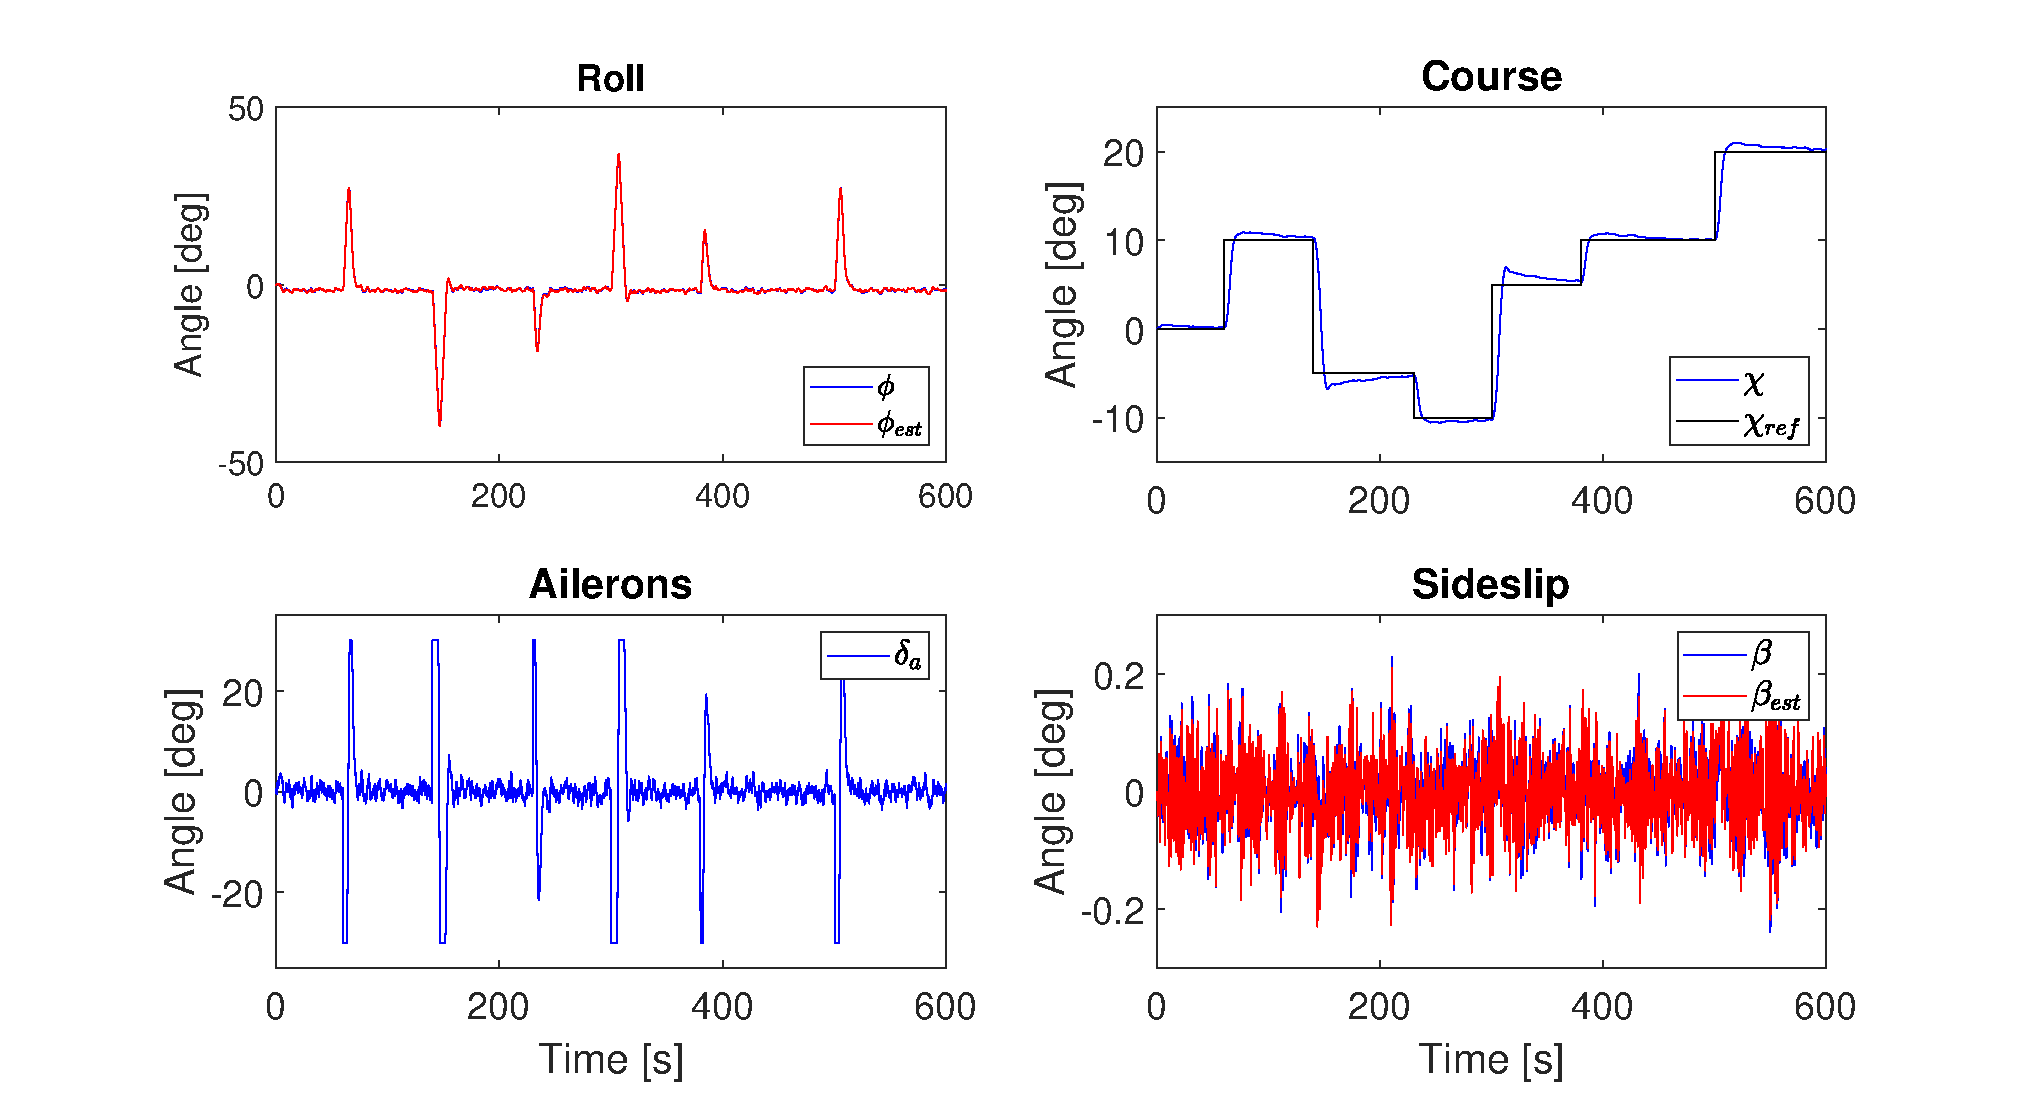
\includegraphics[width=\textwidth]{figures/prob3e.eps}
    \caption{Real versus estimated states with noise-contaminated measurement for roll rate feedback}
    \label{fig:3e}
\end{figure}
\begin{figure}[h!]
    \centering
    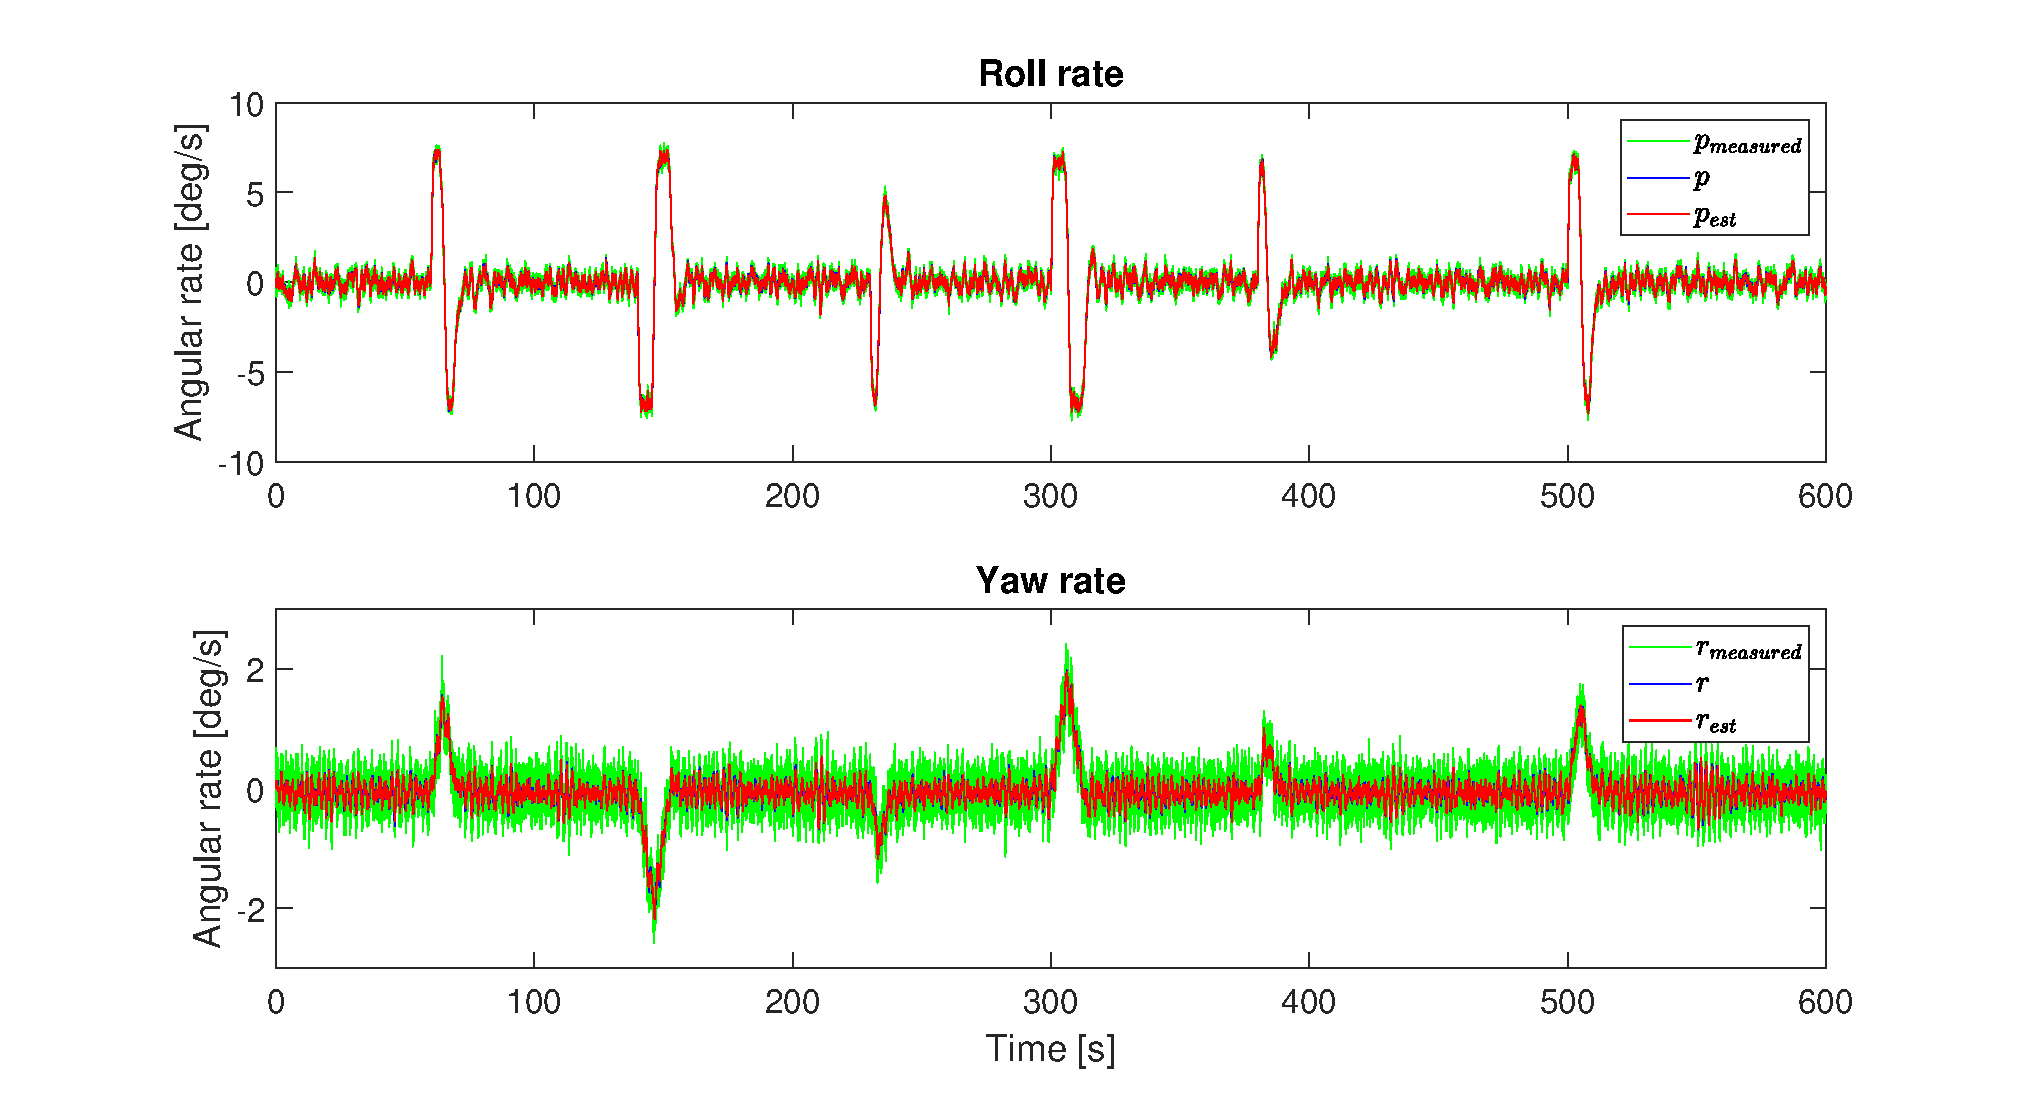
\includegraphics[width=\textwidth]{figures/prob3e_rates.eps}
    \caption{Real versus estimated rates with noise-contaminated measurement for roll rate feedback}
    \label{fig:3e_rates}
\end{figure}



\subsection*{Problem 3.f}
The resulting plots of course, roll, ailerons and sideslip can be seen in Figure \ref{fig:3f} and the plots of roll rate and yaw rate can be found in Figure \ref{fig:3f_rates}. \\

The difference in course control performance can be found by looking at Figure \ref{fig:3e_3f_comparison}, displaying the Aileron input with and without Kalman filtering of the roll rate. As can be seen the Kalman-filtered roll rate causes less oscillations. This corresponds to the theory as the Kalman Filter is meant to decrease the variance of filtered signals.

The bandwidth of the estimator depend on whether you trust the model or the measurement the most. Where a large bandwidth tracks the measurements more which can accentuate the effect of measurement noise and a low bandwidth tracks the model. Generally we want the estimator to have a larger bandwidth than the outer control loop, as it should be faster to ensure stability. We know that the poles of the estimator should be 2-6 times faster than the poles of the plant. 


\begin{figure}[h!]
    \centering
    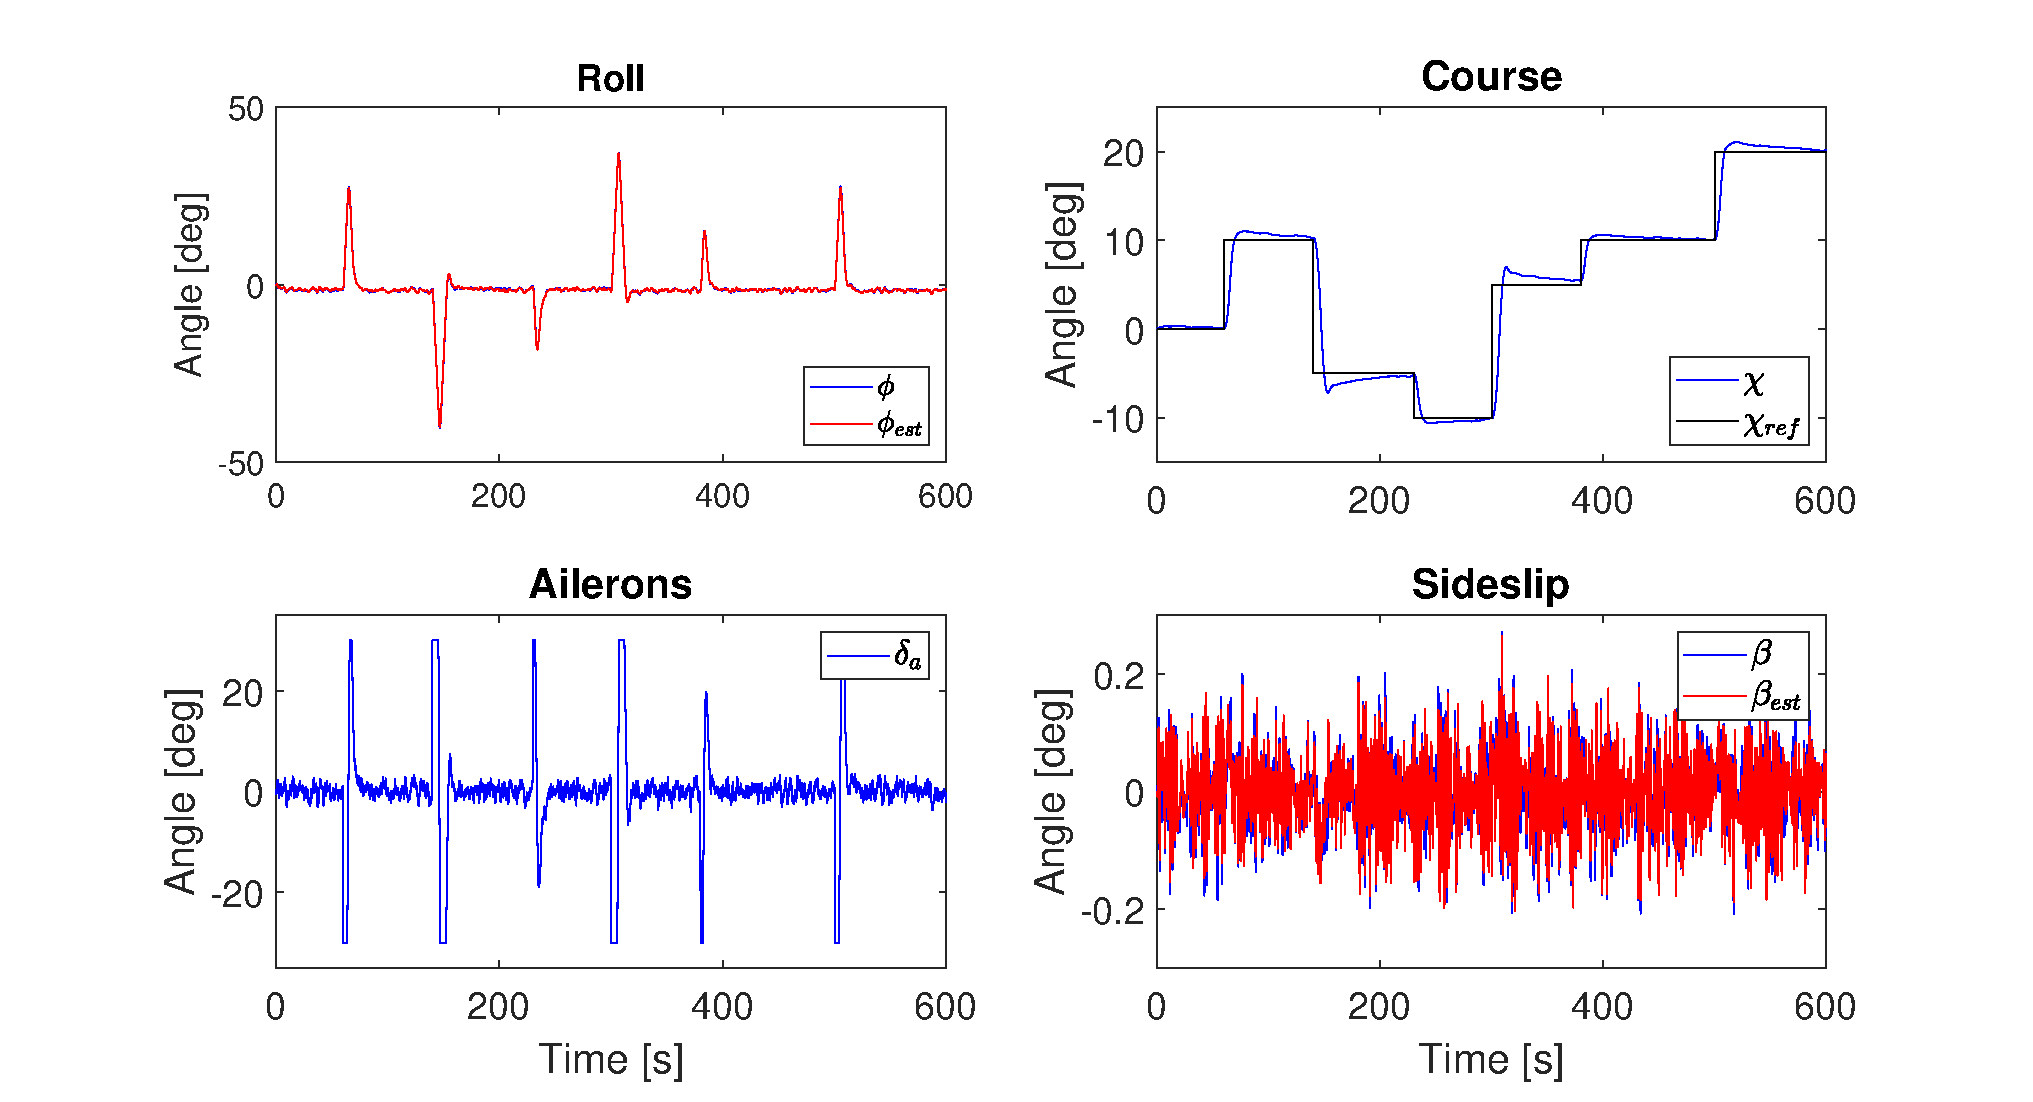
\includegraphics[width=\textwidth]{figures/prob3f.eps}
    \caption{Real versus estimated states with Kalman filtered roll rate feedback}
    \label{fig:3f}
\end{figure}
\begin{figure}[h!]
    \centering
    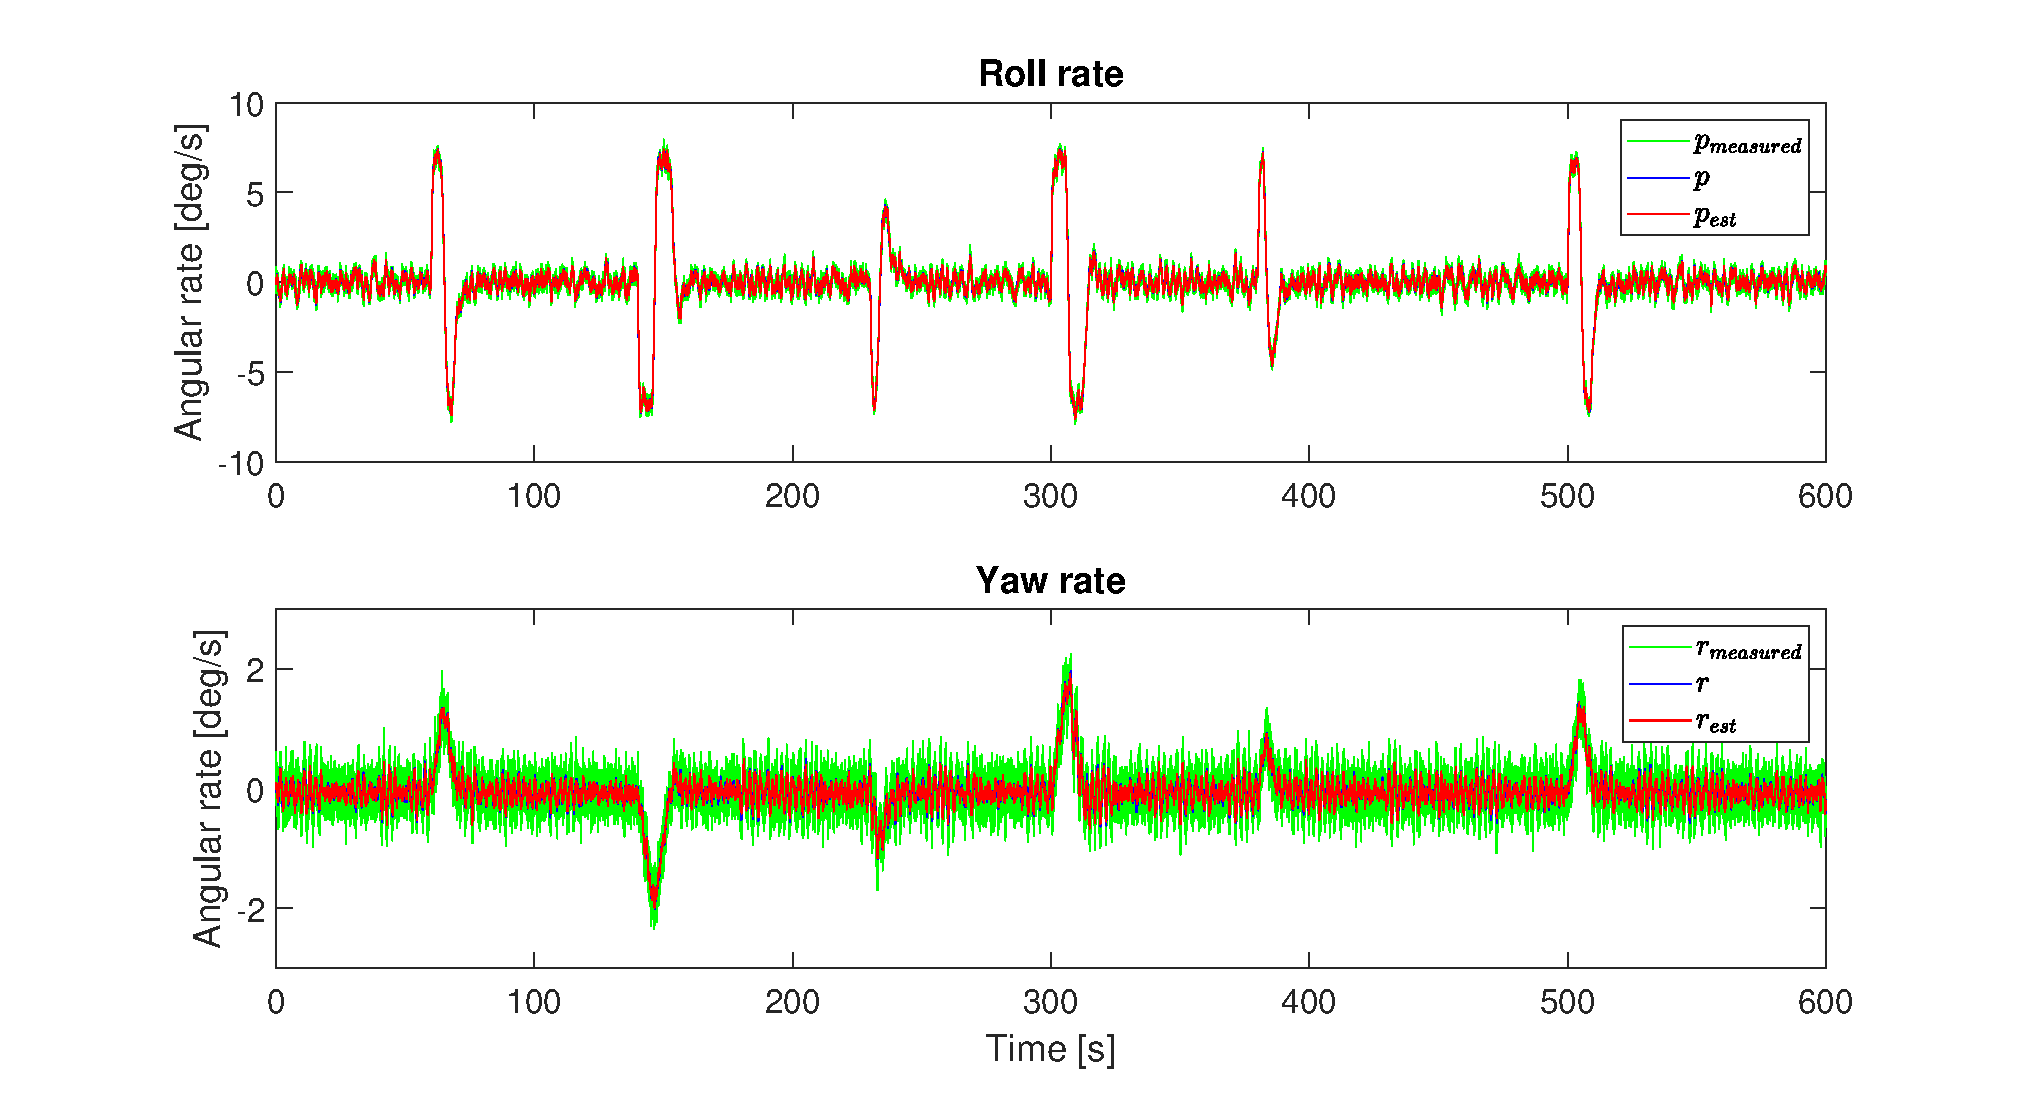
\includegraphics[width=\textwidth]{figures/prob3f_rates.eps}
    \caption{Real versus estimated rates Kalman filtered roll rate feedback}
    \label{fig:3f_rates}
\end{figure}
\begin{figure}[h!]
    \centering
    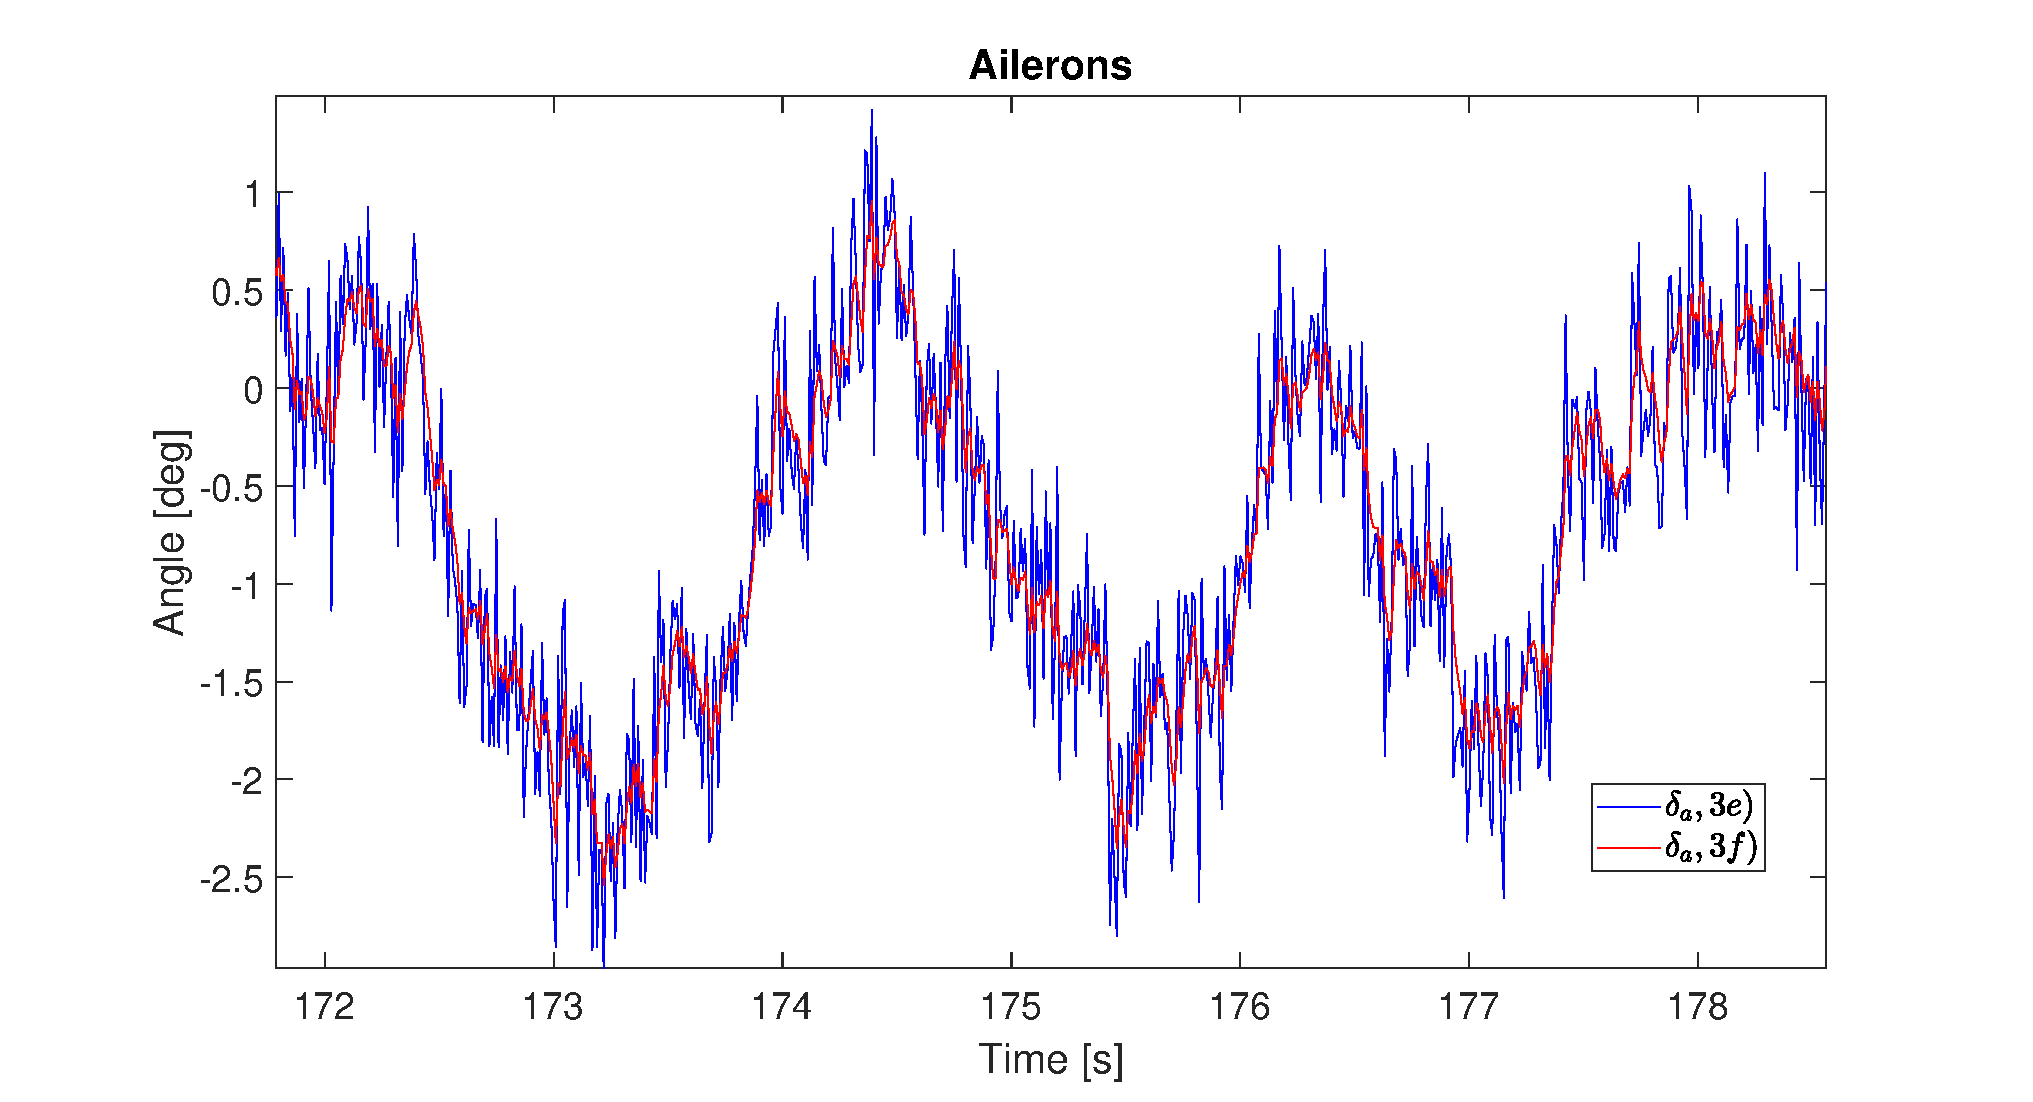
\includegraphics[width=\textwidth]{figures/prob3e_vs_3f.eps}
    \caption{Comparison of the control signals with and without Kalman filtering of the roll rate}
    \label{fig:3e_3f_comparison}
\end{figure}


\subsection*{Problem 3.g}

\begin{figure}[h!]
    \centering
    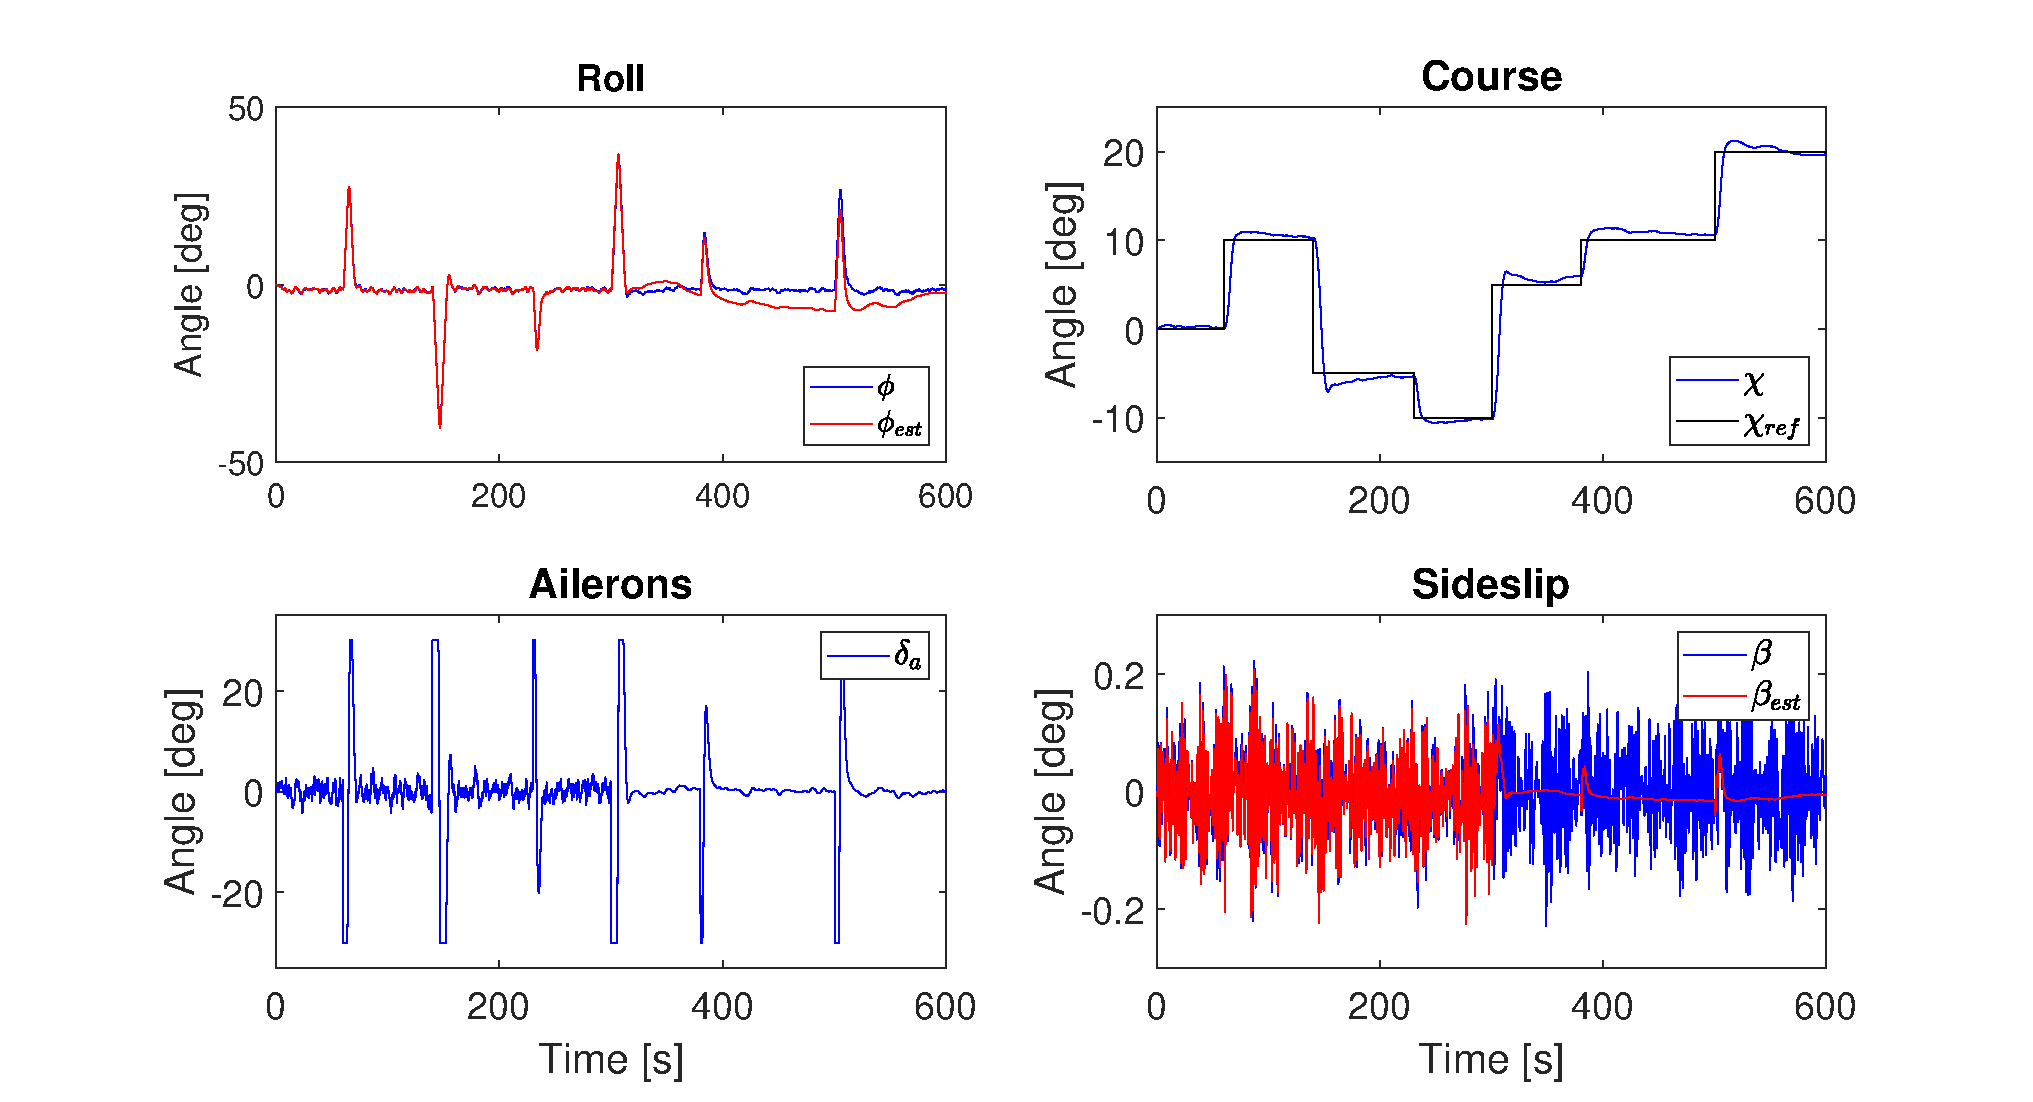
\includegraphics[width=\textwidth]{figures/prob3g.eps}
    \caption{Real versus estimated states with sensory failure after T=300}
    \label{fig:3g}
\end{figure}
\begin{figure}[h!]
    \centering
    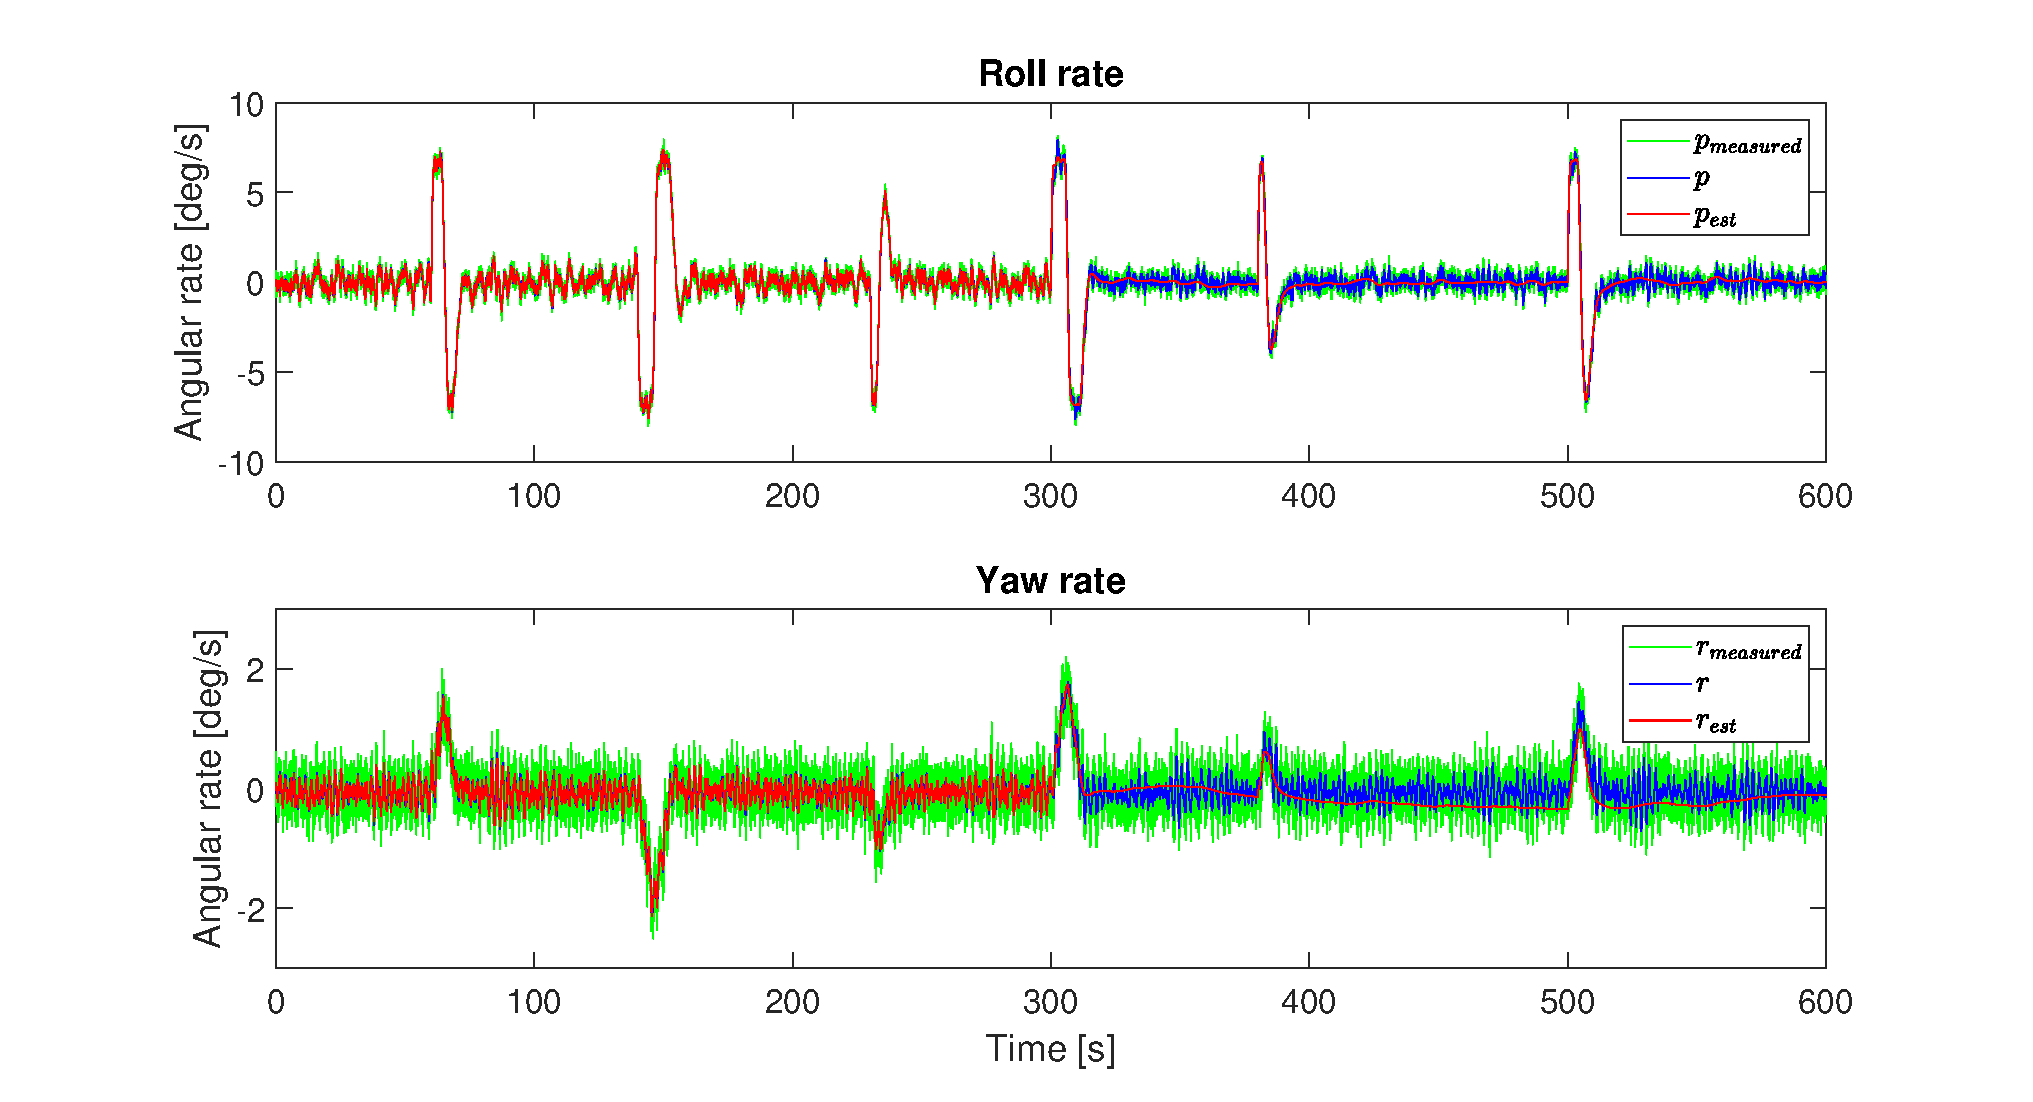
\includegraphics[width=\textwidth]{figures/prob3g_rates.eps}
    \caption{Real versus estimated rates with sensory failure after T=300}
    \label{fig:3g_rates}
\end{figure}

\begin{figure}[h!]
    \centering
    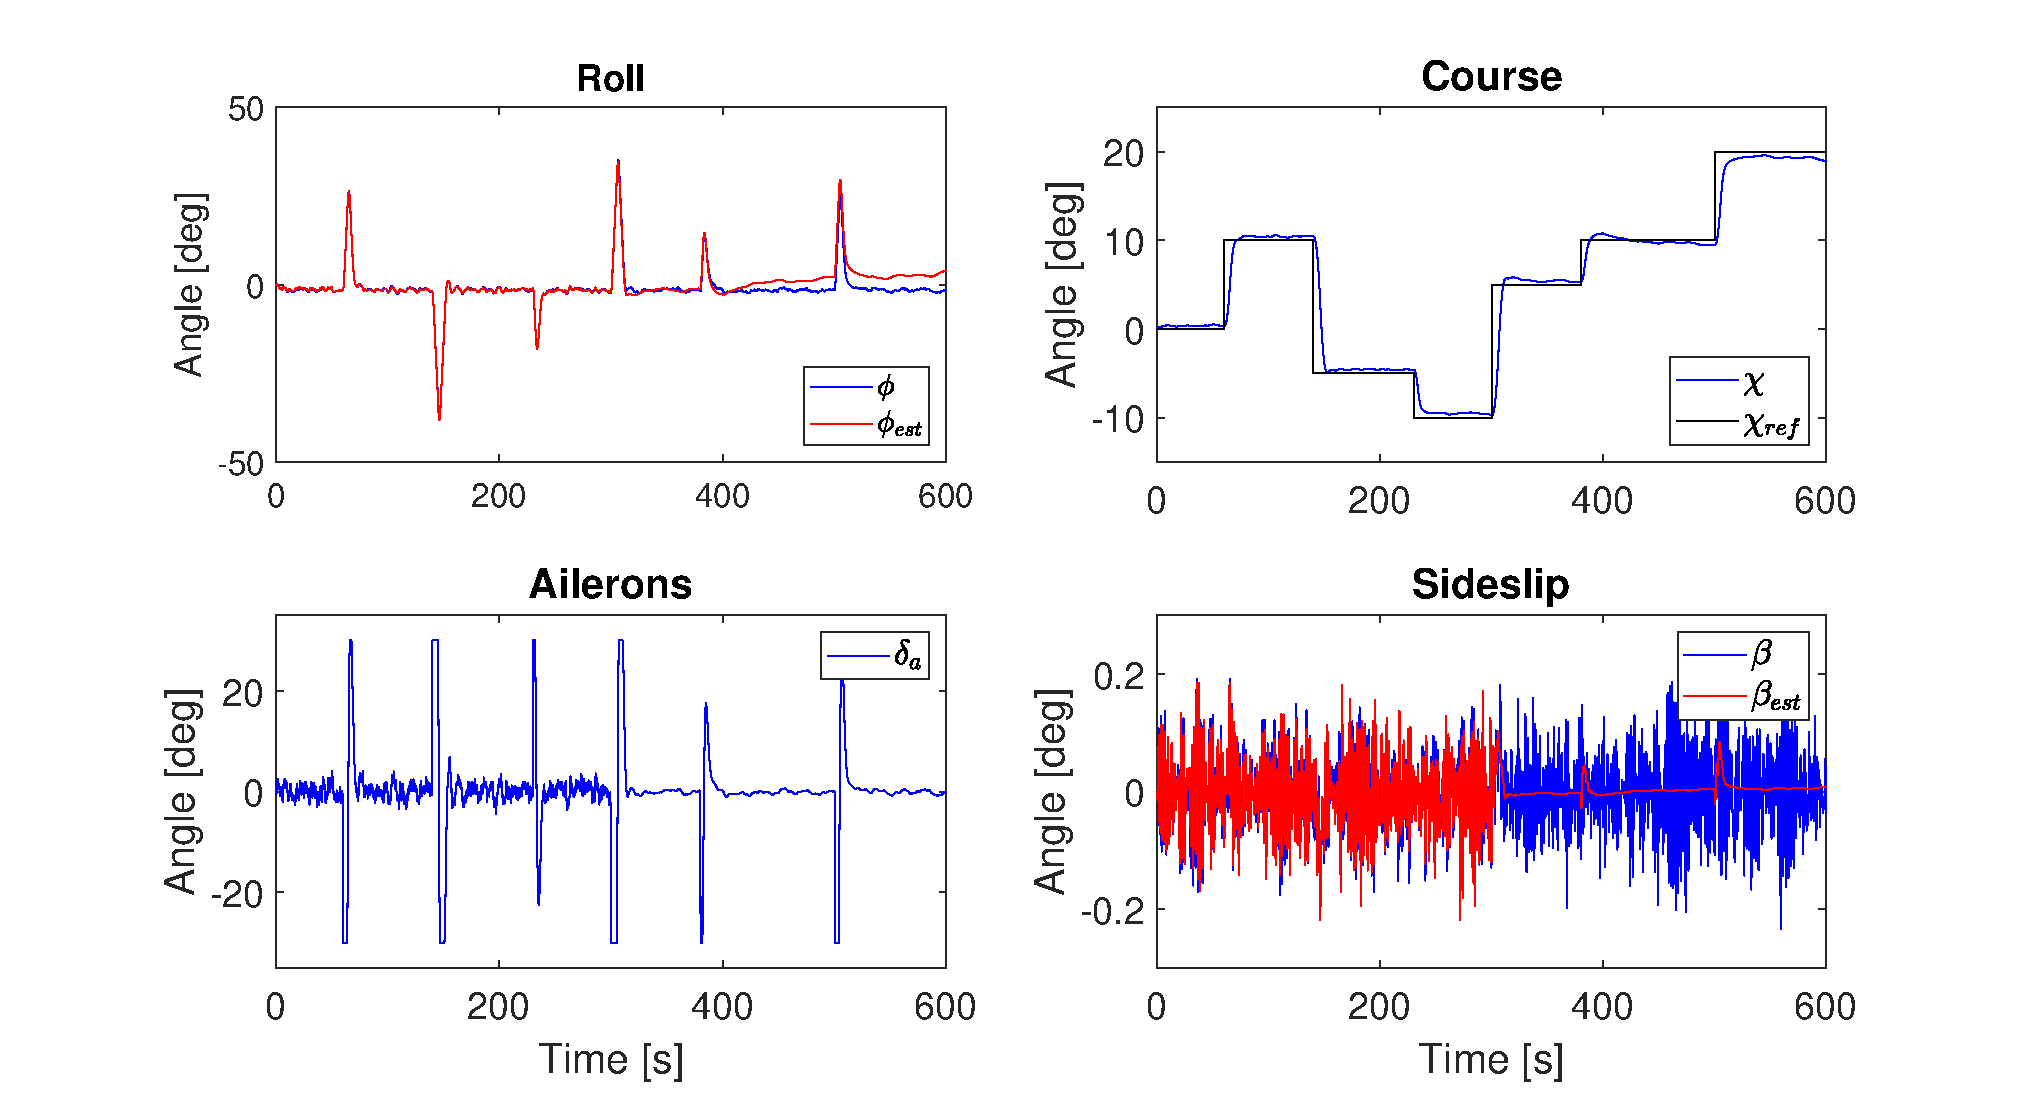
\includegraphics[width=\textwidth]{figures/prob3g_no_integrator.eps}
    \caption{Real versus estimated states with sensory failure after T=300 and no integrator in the outer control loop}
    \label{fig:3g_no_int}
\end{figure}
\begin{figure}[h!]
    \centering
    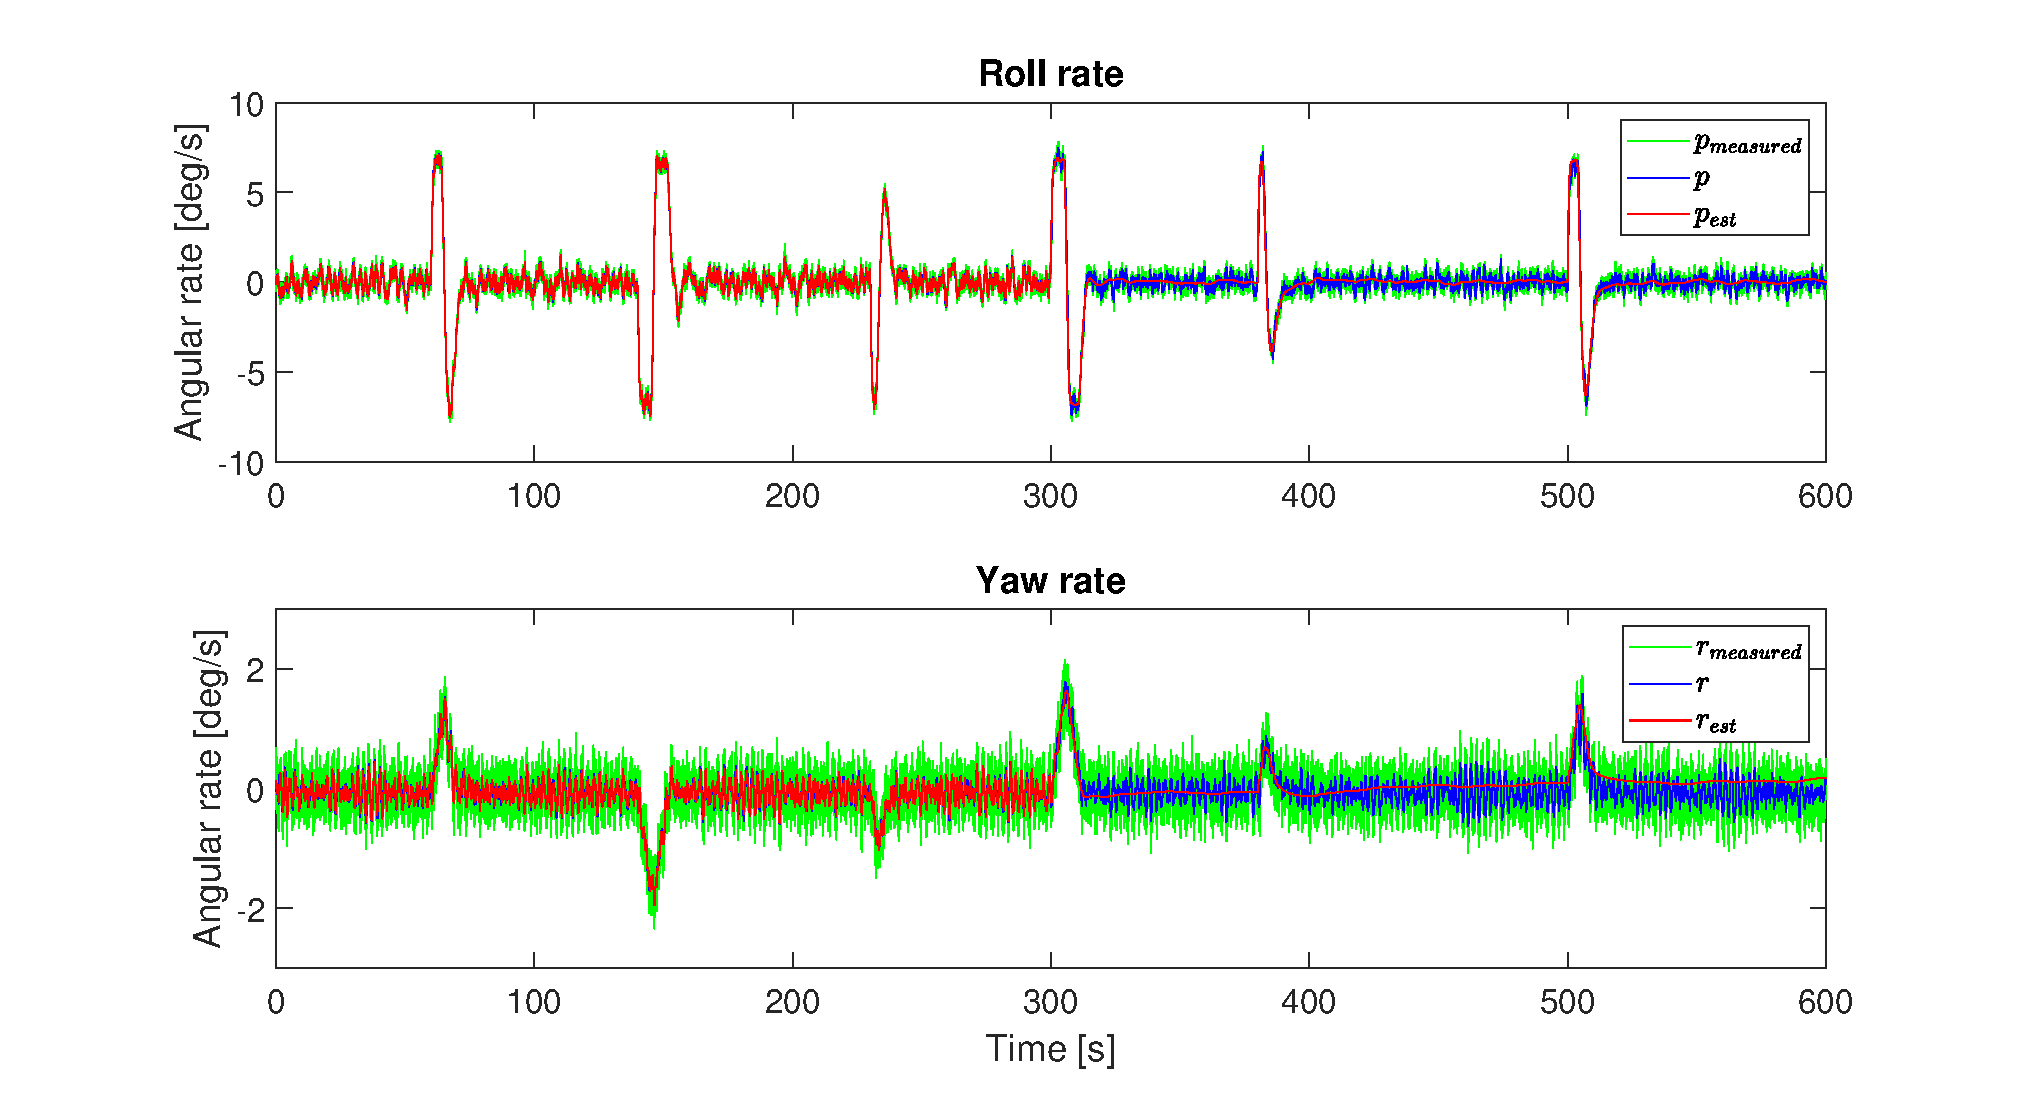
\includegraphics[width=\textwidth]{figures/prob3g_rates_no_integrator.eps}
    \caption{Real versus estimated rates with sensory failure after T=300 and no integrator in the outer control loop}
    \label{fig:3g_rates_no_int}
\end{figure}

Simulating with a sensor failure we see that the results are very similar. This is because the Kalman model is very similar to the "real" model, yielding the system dynamics approximately known. Therefore we do not need the sensor measurements to get decent results. We should also mention that we simulated with and without integral effect on $\chi$. This showed that the feedback on $\chi$ contributes to correcting the drift that would occur when measurements are missing. Both simulations and drift will additionally vary due to the random noise. \\ 
